
\chapter{Természetes számok partíciói}\label{chap:particiok}
\begin{description}
	{\large \item [{Szerző:}] Miklós Dóra (Korszerű módszerek a matematikatanításban, Didaktikai mesteri -- Matematika, 
	II. év)}
\end{description}

\section*{Bevezetés}
\begin{problem}
Hányféleképpen lehet a $7$-et $k\geq1$ pozitív egész szám összegére
felbontani, ha az egymástól csupán az összeadandók sorrendjében eltérő
megoldásokat 
\begin{enumerate}
\item[a)] különbözőnek tekintjük; 
\item[b)] nem tekintjük különbözőnek? 
\item[a)] A $7$-et úgy is elképzelhetjük, mint egy $7$ egység hosszúságú
rudat. 
\begin{center}
\begin{tabular}{|c|c|c|c|c|c|c|}
	\hline 
	&  &  &  &  &  & \tabularnewline
	\hline 
\end{tabular}
\end{center}
Ezt a rudat az egységek mentén $6$ helyen vághatjuk el. Az összes
felvágás úgy kapható meg, ha figyelembe vesszük, hogy minden vágás
helyén vagy vágunk, vagy nem. Így a lehetőségek száma $2^{6}$. 
\item[b)] Írjuk fel a lehetséges felbontásokat:

\begin{minipage}[c]{0.3\textwidth}%
 \hspace{0cm} 
\begin{itemize}
\item[] 7 
\item[] 6 + 1 
\item[] 5 + 2 
\item[] 5 + 1 + 1 
\item[] 4 + 3 
\item[] 4 + 2 + 1 
\item[] 4 + 1 + 1 + 1 
\item[] 3 + 3 + 1 
\end{itemize}
\hspace{0cm} %
\end{minipage}%
\begin{minipage}[c]{0.45\textwidth}%
 \hspace{0cm} 
\begin{itemize}
\item[] 3 + 2 + 2 
\item[] 3 + 2 + 1 + 1 
\item[] 3 + 1 + 1 + 1 + 1 
\item[] 2 + 2 + 2 + 1 
\item[] 2 + 2 + 1 + 1 + 1 
\item[] 2 + 1 + 1 + 1 + 1 + 1 
\item[] 1 + 1 + 1 + 1 + 1 + 1 + 1 
\end{itemize}
\hspace{0cm} %
\end{minipage}

Ez összesen $15$ felbontást jelent. 

\end{enumerate}
\end{problem}
\begin{solution}
Látható, hogy míg az $(5,1,1)$ a b) alpontban egy felbontást jelent,
addig az a) alpontban ennek három felel meg: $(5,1,1)$, $(1,5,1)$,
$(1,1,5)$. 
\end{solution}

\section*{Természetes szám partíciója}
\begin{definition}{def:particio}
Az $n\geq1$ természetes szám partíciójának nevezünk minden olyan
$n=\lambda_{1}+\lambda_{2}+...+\lambda_{k}$ előállítást, ahol $\lambda_{1}\geq\lambda_{2}\geq\dots\geq\lambda_{k}>0$.\par Jelölés:
$\lambda=(\lambda_{1},\lambda_{2},...,\lambda_{k})$.
\end{definition}
Jelöljük $p(n)$-nel az $n$ összes partícióinak számát. 
\begin{example}
\begin{multicols}{3} $p(3)=3:$ 
\begin{align*}
 & 3\\
 & 2+1\\
 & 1+1+1
\end{align*}
\par $p(4)=5$: 
\begin{align*}
 & 4\\
 & 3+1\\
 & 2+2\\
 & 2+1+1\\
 & 1+1+1+1
\end{align*}
$p(5)=7$: 
\begin{align*}
 & 5\\
 & 4+1\\
 & 3+2\\
 & 3+1+1\\
 & 2+2+1\\
 & 2+1+1+1\\
 & 1+1+1+1+1
\end{align*}
\end{multicols}
\end{example}

\section*{Partíciók szemléltetése: Young--diagram}

A partíciók szemléltethetőek a következőképpen:
\begin{itemize}
\item Legyen $\lambda=(\lambda_{1},\lambda_{2},...,\lambda_{k})$ partíció. 
\item Az $i$. oszlopba $\lambda_{i}$ darab négyzetet rajzolunk. 
\end{itemize}
\begin{example}
Vegyük a következő partíciókat: \begin{multicols}{2} \hspace{1.5cm}
$(5,3,1,1)$ \begin{center} 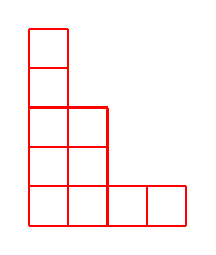
\begin{tikzpicture} \draw[step=0.5cm,
red, thick] (0,1.5) grid (0.5,2.5); \draw[step=0.5cm, red, thick]
(0,0.5) grid (1,1.5); \draw[step=0.5cm, red, thick] (0,0) grid
(2,0.5); \end{tikzpicture} \end{center} \hspace{1cm} 
\[
(4,2,2,1,1)
\]
\begin{center} 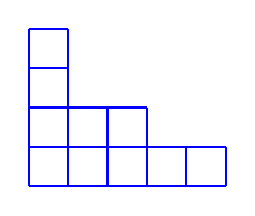
\begin{tikzpicture} \draw[step=0.5cm, blue, thick]
(0,1) grid (0.5,2); \draw[step=0.5cm, blue, thick] (0,0.5) grid
(1.5,1); \draw[step=0.5cm, blue, thick] (0,0) grid (2.5,0.5); \end{tikzpicture}
\end{center} \end{multicols}\par Megvizsgálva a két partíciót az
alábbi észrevételt állapíthatjuk meg:\par %
\begin{minipage}[c]{0.4\textwidth}%
 \hspace{0cm} 
\begin{center}
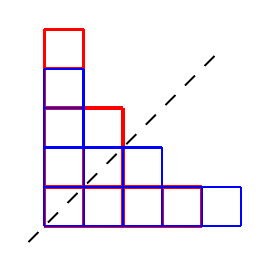
\begin{tikzpicture}
            \draw [line width=0.6pt,dash pattern=on 5pt off 5pt] (-0.2,-0.2)-- (2.2,2.2);
            \draw[step=0.5cm, red, very  thick] (0,1.5) grid (0.5,2.5);
            \draw[step=0.5cm, red, very  thick] (0,0.5) grid (1,1.5);
            \draw[step=0.5cm, red, very  thick] (0,0) grid (2,0.5);
            \draw [line width=0.6pt,dash pattern=on 5pt off 5pt] (-0.2,-0.2)-- (2.2,2.2);
            \draw[step=0.5cm, blue,  thick] (0,1) grid (0.5,2);
            \draw[step=0.5cm, blue,  thick] (0,0.5) grid (1.5,1);
            \draw[step=0.5cm, blue, thick] (0,0) grid (2.5,0.5);
        \end{tikzpicture} 
\par\end{center}%
\end{minipage}%
\begin{minipage}[c]{0.5\textwidth}%
 Az $(5,3,1,1)$ és $(4,2,2,1,1)$ partíciók Young-diagramja között
észrevehető az a kapcsolat, hogy egymás szimmetrikusai az első szögfelezőre
nézve. %
\end{minipage}
\end{example}
\begin{definition}{def:Young-diagram}
Ha egy $\lambda$ partíció Young-diagramját az első szögfelezőre
tükrözzük, akkor a kapott partíciót a $\lambda$ konjugáltjának nevezzük. 
\end{definition}
\begin{example}
 \hspace{0.1cm}\par \begin{multicols}{2} Adott a $(7,5,2,2,1)$
partíció. \begin{center} 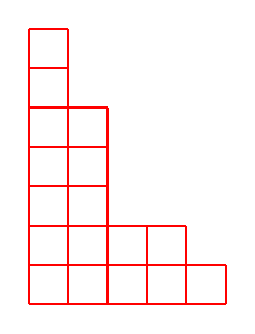
\begin{tikzpicture} \draw[step=0.5cm,
red, thick] (0,2.5) grid (0.5,3.5); \draw[step=0.5cm, red, thick]
(0,1) grid (1,2.5); \draw[step=0.5cm, red, thick] (0,0.5) grid
(2,1); \draw[step=0.5cm, red, thick] (0,0) grid (2.5,0.5); \end{tikzpicture}
\end{center}\par A konjugáltja: $(5,4,2,2,2,1,1)$\par \begin{center}
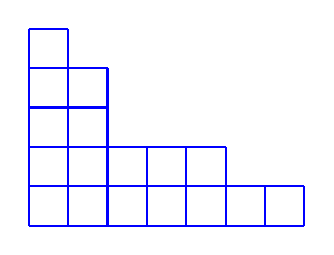
\begin{tikzpicture} \draw[step=0.5cm, blue, thick] (0,2) grid
(0.5,2.5); \draw[step=0.5cm, blue, thick] (0,1) grid (1,2); \draw[step=0.5cm,
blue, thick] (0,0.5) grid (2.5,1); \draw[step=0.5cm, blue, thick]
(0,0) grid (3.5,0.5); \end{tikzpicture} \end{center} \end{multicols} 
\end{example}

\section*{Történelmi kitekintés}

A partíció problémájával először valamikor 1674-ben találkozunk, amikor
Gottfried Leibniz egy Bernoullinak írt levelében azt a kérdést teszi
fel, hogy a természetes számokat hogyan lehet szintén természetes
számok összegeként felbontani. Egészen 6-ig meg is válaszolta saját
kérdését, majd levonta azt a helytelen következtetést, hogy a felbontások
száma mindig prím. Hamar rájött a hibájára, hiszen már $p(7)=15$.

Ezt követően az első komolyabb észrevételeket Leonhard Eulerhez kapcsoljuk
(18. század), aki lényeges összefüggéseket vett észre a partíciókat
kapcsolatosan. Például tőle származtatjuk a következő tételt: tetszőleges
$n$ esetén a páratlan számokból felírt partíciók száma megegyezik
a csak különböző számokkal felírt partíciók számával. Emellett a partíciók
számára felírt generátorfüggvényt is az ő nevéhez kapcsoljuk.

Sokáig dolgoztak azon, hogy egzakt képletet adjanak meg a partíciók
számára, de helyett egy elég jó becslést sikerült megadni. Az indiai
Srínivásza Rámánudzsan, valamint professzora Godfrey Harold Hardy,
akik 1918-as publikációjukban a következő közelítést adták meg a partíciók
számára: 
\[
p(n)\sim\frac{1}{4n\cdot\sqrt{3}}\cdot e^{\pi\sqrt{2n/3}}.
\]
Ezen a felfedezésen alapszik "Az ember, aki ismerte a végtelent"
(2015) film, amely bemutatja Rámánudzsan felfedezését és életét.

\section*{Generátorfüggvény}

Habár egzakt képletet nem ismerünk a partíciók számára, a generátorfüggvénye
könnyen előállítható. Célunk olyan polinomiális függvény megadása,
ahol az $x^{n}$ tagnak az együtthatója $p(n)$. Ehhez az $n=k_{1}\cdot1+k_{2}\cdot2+k_{3}\cdot3+\dots+k_{n}\cdot n$
alakú partíciók előállítása a célunk, ahol $k_{i}\geq0$ és azt mutatja
meg, hogy az adott számból hány szerepel a partícióban.

Először a tiszta partíciók előállítására törekszünk, mely alatt olyan
partíciókat értünk, ahol a felírásban csak egyforma számok szerepelnek.
Ezekhez az alábbi összegzéseket vesszük: 
\[
1+x^{1}+x^{1+1}+x^{1+1+1}+x^{1+1+1+1}+\dots=1+x^{1\cdot1}+x^{2\cdot1}+x^{3\cdot1}+x^{4\cdot1}+\dots
\]

\[
1+x^{2}+x^{2+2}+x^{2+2+2}+x^{2+2+2+2}+\dots=1+x^{1\cdot2}+x^{2\cdot2}+x^{3\cdot2}+x^{4\cdot2}+\dots
\]

%\[
%1+ x^{3}+x^{3 + 3}+x^{3 + 3 + 3}+x^{3+ 3+ 3 + 3} + \dots = 1+x^{1 \cdot 3}+x^{2 \cdot 3}+x^{3 \cdot 3} + x^{4 \cdot 3}+ \dots
%\]

\begin{center}
$\dots$ 
\par\end{center}

\[
1+x^{n}+x^{n+n}+x^{n+n+n}+x^{n+n+n+n}+\dots=1+x^{1\cdot n}+x^{2\cdot n}+x^{3\cdot n}+x^{4\cdot n}+\dots
\]
A vegyes partíciókat, ahol már tetszőleges számok jelenhetnek meg
ezek szorzásából kapjuk: 
\begin{align*}
 & (1+x^{1\cdot1}+x^{2\cdot1}+x^{3\cdot1}+\dots)\cdot(1+x^{1\cdot2}+x^{2\cdot2}+x^{3\cdot2}+\dots)\cdot\\
 & \cdot(1+x^{1\cdot3}+x^{2\cdot3}+x^{3\cdot3}+\dots)\cdot...\cdot(1+x^{1\cdot n}+x^{2\cdot n}+x^{3\cdot n}+\dots)=\\
 & =\frac{1}{1-x}\cdot\frac{1}{1-x^{2}}\cdot\frac{1}{1-x^{3}}\cdot...\cdot\frac{1}{1-x^{n}}=\prod\limits_{k=1}^{n}\frac{1}{1-x^{k}}
\end{align*}
Ennek a szorzat egy tetszőleges tagja: $x^{k_{1}\cdot1+k_{2}\cdot2+k_{3}\cdot3+...+k_{n}\cdot n}.$
Így a generátorfüggvény általános alakja: 
\[
\boxed{\sum\limits_{n=0}^{\infty}p(n)\cdot x^{n}=\prod\limits_{k=1}^{n}\frac{1}{1-x^{k}}}
\]


\section*{Partíciók feltételekkel}

A Young-diagramokat tekintve a diagram magasságára és szélességére
vonatkozóan plusz kikötéseket szabhatunk meg.

\vspace{0.5cm}

\begin{minipage}[c]{0.5\textwidth}%
\vspace{0.2cm}

\begin{center}
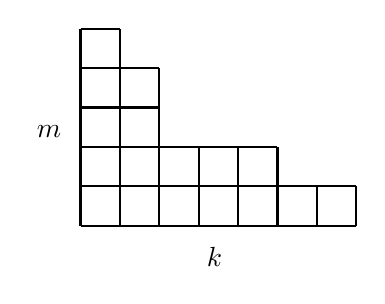
\begin{tikzpicture}
        \draw[step=0.5cm, black, thick] (0,2) grid (0.5,2.5);
        \draw[step=0.5cm, black, thick] (0,1) grid (1,2);
        \draw[step=0.5cm, black, thick] (0,0.5) grid (2.5,1);
        \draw[step=0.5cm, black, thick] (0,0) grid (3.5,0.5);
        \draw[color=black] (-0.4,1.2) node {$m$};
         \draw[color=black] (1.7,-0.4) node {$k$};
    \end{tikzpicture} 
\par\end{center}%
\end{minipage}%
\begin{minipage}[c]{0.5\textwidth}%
 Vezessük be az alábbi jelöléseket:

\vspace{0.1cm}

\textcolor{black}{m} - a partíció legnagyobb tagja

\vspace{0.1cm}

\textcolor{black}{k} - ahány számból áll a partíció %
\end{minipage}A következőkben egy-egy ilyen típusát vizsgáljuk meg a partícióknak.

\hspace{0.1cm}

\textbf{1. Partíciók, melyeket $k$ szám alkot:}

\hspace{0cm}

Jelölje $p(n,k)$ azon partícióknak a számát, melyeket $k$ darab
szám alkot. 
\begin{example}
Ha $n=8$ és $k=2$, akkor $p(8,2)=4.$ %\vspace{0.2cm}
\begin{center}
{\setlength{\tabcolsep}{12pt}
	\begin{tabular}{cccc}
		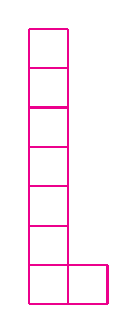
\begin{tikzpicture} \draw[step=0.5cm, magenta,
			thick] (0,0.5) grid (0.5,3.5); \draw[step=0.5cm, magenta, thick]
			(0,0) grid (1,0.5); \end{tikzpicture} & 
		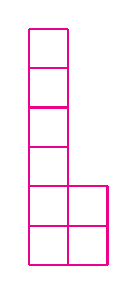
\begin{tikzpicture}
			\draw[step=0.5cm, magenta, thick] (0,1) grid (0.5,3); \draw[step=0.5cm,
			magenta, thick] (0,0) grid (1,1); \end{tikzpicture} &
		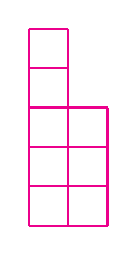
\begin{tikzpicture} \draw[step=0.5cm, magenta, thick] (0,1.5)
			grid (0.5,2.5); \draw[step=0.5cm, magenta, thick] (0,0) grid (1,1.5);
		\end{tikzpicture} &
		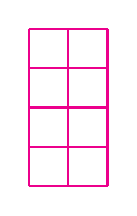
\begin{tikzpicture} \draw[step=0.5cm,
			magenta, thick] (0,0) grid (1,2); \end{tikzpicture} \tabularnewline
		$(7,1)$ & $(6,2)$ &	$(5,3)$ & $(4,4)$ 
	\end{tabular}
}
\end{center}
\end{example}
A következőkben azt szeretnénk megvizsgálni, hogy mennyi $p(9,3)$
értéke a korábbi példák alapján. Arra jöhetünk rá, hogy kétféle csoportba
oszthatjuk ezeket a partíciókat: azok amelyekben van 1-es és azok
amelyekben nincs.

Azokat, ahol van 1-es megkaphatjuk a $p(8,2)$ partíciókból úgy, hogy
a diagramokat kiegészítjük jobbról még egy 1 magasságú oszloppal:
\begin{center}
{\setlength{\tabcolsep}{12pt}
	\begin{tabular}{cccc}
		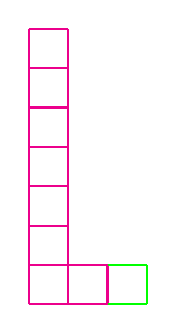
\begin{tikzpicture}
			\draw[step=0.5cm, magenta, thick] (0,0.5) grid (0.5,3.5);
			\draw[step=0.5cm, magenta, thick] (0,0) grid (1,0.5);
			\draw[step=0.5cm, green, thick] (1,0) grid (1.5,0.5);
		\end{tikzpicture} & 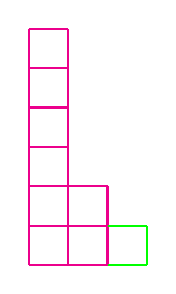
\begin{tikzpicture}
			\draw[step=0.5cm, magenta, thick] (0,1) grid (0.5,3);
			\draw[step=0.5cm, magenta, thick] (0,0) grid (1,1);
			\draw[step=0.5cm, green, thick] (1,0) grid (1.5,0.5);
		\end{tikzpicture} & 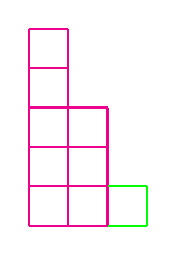
\begin{tikzpicture}
			\draw[step=0.5cm, magenta, thick] (0,1.5) grid (0.5,2.5);
			\draw[step=0.5cm, magenta, thick] (0,0) grid (1,1.5);
			\draw[step=0.5cm, green, thick] (1,0) grid (1.5,0.5);
		\end{tikzpicture} & 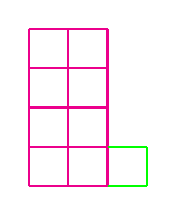
\begin{tikzpicture}
			\draw[step=0.5cm, magenta, thick] (0,0) grid (1,2);
			\draw[step=0.5cm, green, thick] (1,0) grid (1.5,0.5);
		\end{tikzpicture} \tabularnewline
		$(7,1,\textcolor{green}{1})$ & $(6,2,\textcolor{green}{1})$	& $(5,3,\textcolor{green}{1})$ & $(4,4,\textcolor{green}{1})$
	\end{tabular}
}
\end{center}


Ugyanakkor azokat, amelyekben nem szerepel 1-es úgy kaphatjuk meg,
hogy a $p(6,3)$ partíciói esetén, a diagramok minden oszlopára még
egy plusz négyzetet teszünk. Ez az alábbi ábrákon látható:

\begin{center}
{\setlength{\tabcolsep}{12pt}
	\begin{tabular}{ccc}
	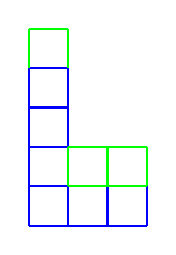
\begin{tikzpicture}
		\draw[step=0.5cm, blue, thick] (0,0.5) grid (0.5,2);
		\draw[step=0.5cm, blue, thick] (0,0) grid (1.5,0.5);
		\draw[step=0.5cm, green, thick] (0,2) grid (0.5,2.5);
		\draw[step=0.5cm, green, thick] (0.5,0.5) grid (1.5,1);
	\end{tikzpicture} & 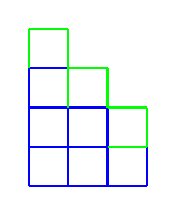
\begin{tikzpicture}
		\draw[step=0.5cm, blue, thick] (0,1) grid (0.5,1.5);
		\draw[step=0.5cm, blue, thick] (0,0.5) grid (1,1);
		\draw[step=0.5cm, blue, thick] (0,0) grid (1.5,0.5);
		\draw[step=0.5cm, green, thick] (1,0.5) grid (1.5,1);
		\draw[step=0.5cm, green, thick] (0.5,1) grid (1,1.5);
		\draw[step=0.5cm, green, thick] (0,1.5) grid (0.5,2);
	\end{tikzpicture} & 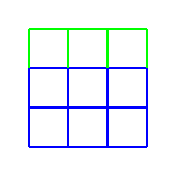
\begin{tikzpicture}
		\draw[step=0.5cm, blue, thick] (0,0) grid (1.5,1);
		\draw[step=0.5cm, green, thick] (0,1) grid (1.5,1.5);
	\end{tikzpicture} \tabularnewline
	 $(\textcolor{green}{5},\textcolor{green}{2},\textcolor{green}{2})$ 
	& $(\textcolor{green}{4},\textcolor{green}{3},\textcolor{green}{2})$
	& $(\textcolor{green}{3},\textcolor{green}{3},\textcolor{green}{3})$
	\end{tabular}
}
\end{center}

\vspace{0.3cm}

Tehát $p(9,3)=p(8,2)+p(6,3)=4+3=7.$ Tetszőleges $n,k\in\mathbb{N}$,
$k\leq n$ számok esetén is felírható egy ehhez hasonló rekurzív összefüggés
a $p(n,k)$ értékére. Ezt a következő tételben szemléltetjük. 
\begin{theorem}{thm:part1}
Tetszőleges $n$ és $k\leq n$ természetes számok esetén teljesül,
hogy 
\[
p(n,k)=p(n-1,k-1)+p(n-k,k).
\]
\end{theorem}
\begin{solution}
Alapötlet: 
\[
p(n,k)=\textcolor{magenta}{\underbrace{p(n-1, k-1)}_{\textrm{tartalmaz 1-est}}}+\textcolor{blue}{ \underbrace{p(n-k,k)}_{\textrm{nem tartalmaz 1-est}}}
\]
\end{solution}
\hspace{0.1cm}

\textbf{2. Partíciók, melyek legnagyobb értéke $m$:}

\hspace{0.1cm}

Jelölje $q(n,m)$ azon partíciók száma, melyek legnagyobb értéke $m$. 
\begin{example}
Ha $n=9$ és $m=3$, akkor $q(9,3)=7$.\par \vspace{0.2cm}
\par \hspace{1cm} 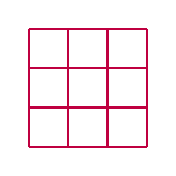
\begin{tikzpicture} \draw[step=0.5cm, purple,
thick] (0,0) grid (1.5,1.5); \end{tikzpicture} \hspace{0.3cm} 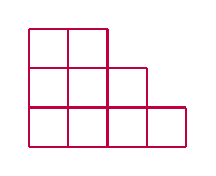
\begin{tikzpicture}
\draw[step=0.5cm, purple, thick] (0,1) grid (1,1.5); \draw[step=0.5cm,
purple, thick] (0,0.5) grid (1.5,1); \draw[step=0.5cm, purple,
thick] (0,0) grid (2,0.5); \end{tikzpicture} \hspace{0.3cm} 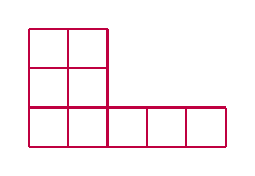
\begin{tikzpicture}
\draw[step=0.5cm, purple, thick] (0,0.5) grid (1,1.5); \draw[step=0.5cm,
purple, thick] (0,0) grid (2.5,0.5); \end{tikzpicture} \hspace{0.3cm}
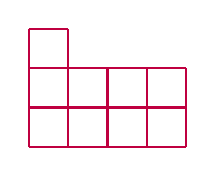
\begin{tikzpicture} \draw[step=0.5cm, purple, thick] (0,1) grid
(0.5,1.5); \draw[step=0.5cm, purple, thick] (0,0) grid (2,1); \end{tikzpicture}\par \hspace{1.2cm}
$(3,3,3)$ \hspace{0.8cm} $(3,3,2,1)$ \hspace{0.95cm} $(3,3,1,1,1)$
\hspace{0.95cm} $(3,2,2,2)$\par \vspace{0.2cm}
\par \hspace{0.9cm} 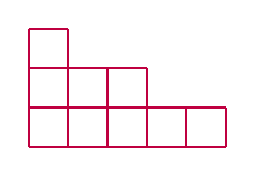
\begin{tikzpicture} \draw[step=0.5cm, purple,
thick] (0,1) grid (0.5,1.5); \draw[step=0.5cm, purple, thick]
(0,0.5) grid (1.5,1); \draw[step=0.5cm, purple, thick] (0,0) grid
(2.5,0.5); \end{tikzpicture} \hspace{0.3cm} 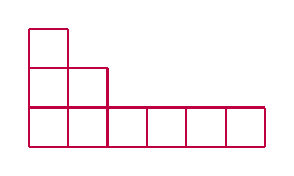
\begin{tikzpicture}
\draw[step=0.5cm, purple, thick] (0,1) grid (0.5,1.5); \draw[step=0.5cm,
purple, thick] (0,0.5) grid (1,1); \draw[step=0.5cm, purple, thick]
(0,0) grid (3,0.5); \end{tikzpicture} \hspace{0.3cm} 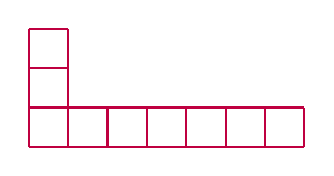
\begin{tikzpicture}
\draw[step=0.5cm, purple, thick] (0,0.5) grid (0.5,1.5); \draw[step=0.5cm,
purple, thick] (0,0) grid (3.5,0.5); \end{tikzpicture}\par \hspace{1.3cm}
$(3,2,2,1,1)$ \hspace{1.15cm} $(3,2,1,1,1,1)$ \hspace{1.25cm}
$(3,1,1,1,1,1,1)$ 

\vspace*{0.1cm}

Észrevehetjük, hogy $p(9,3)$ partíciói konjugáltjai a $q(9,3)$ partícióknak,
valamint 
\[
p(9,3)=q(9,3).
\]
Ez alapján megfogalmazható az alábbi tétel.
\end{example}
\begin{theorem}{thm:part2}
Tetszőleges $n$ és $k\leq n$ természetes számokra igaz a következő: $p(n,k)=q(n,k).$
\end{theorem}
\hspace{0cm}

\textbf{3. Partíciók, melyeket $k$ szám alkot és a legnagyobb érték
kisebb vagy egyenlő, mint $m$:}

\hspace{0.1cm}

Jelölje $s(n,m,k)$ az $n$ azon partícióinak a száma, melyek legnagyobb
értéke kisebb vagy egyenlő, mint $m$ és a partíció $k$ értékből
áll. 
\begin{example}
Ha $n=10$, $m=5$, $k=6$, akkor $s(10,5,6)=5$.\par \vspace{0.1cm}
\par \hspace{0.6cm} 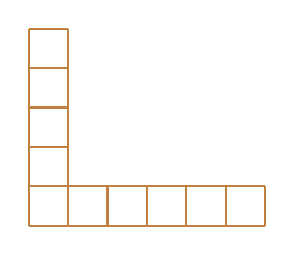
\begin{tikzpicture} \draw[step=0.5cm, brown,
thick] (0,0.5) grid (0.5,2.5); \draw[step=0.5cm, brown, thick]
(0,0) grid (3,0.5); \end{tikzpicture} \hspace{0.5cm} 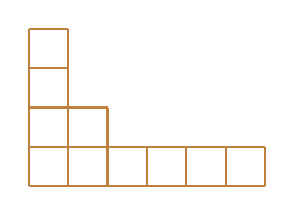
\begin{tikzpicture}
\draw[step=0.5cm, brown, thick] (0,1) grid (0.5,2); \draw[step=0.5cm,
brown, thick] (0,0.5) grid (1,1); \draw[step=0.5cm, brown, thick]
(0,0) grid (3,0.5); \end{tikzpicture} \hspace{0.5cm} 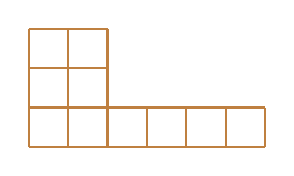
\begin{tikzpicture}
\draw[step=0.5cm, brown, thick] (0,0.5) grid (1,1.5); \draw[step=0.5cm,
brown, thick] (0,0) grid (3,0.5); \end{tikzpicture}\par \hspace{0.9cm}
$(5,1,1,1,1,1,1)$ \hspace{1.25cm} $(4,2,1,1,1,1)$ \hspace{1.4cm}
$(3,3,1,1,1,1)$\par \hspace{2.5cm} 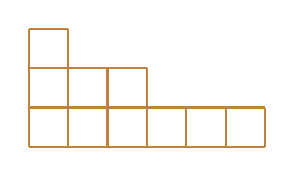
\begin{tikzpicture} \draw[step=0.5cm,
brown, thick] (0,1) grid (0.5,1.5); \draw[step=0.5cm, brown, thick]
(0,0.5) grid (1.5,1); \draw[step=0.5cm, brown, thick] (0,0) grid
(3,0.5); \end{tikzpicture} \hspace{0.5cm} 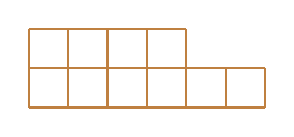
\begin{tikzpicture} \draw[step=0.5cm,
brown, thick] (0,0.5) grid (2,1); \draw[step=0.5cm, brown, thick]
(0,0) grid (3,0.5); \end{tikzpicture}\par \hspace{2.95cm} $(3,2,2,1,1,1)$
\hspace{1.4cm} $(2,2,2,2,1,1)$ 
\end{example}

\section*{Alkalmazás}
\begin{problem}
Határozzuk meg az 6 csúccsal rendelkező fák lehetséges alakjait! 
\end{problem}
\begin{solution}
Vegyük számba előbb a fák legismertebb tulajdonságait: 
\begin{itemize}
\item A fák körmentes és összefüggő gráfok. 
\item Egy $n$ csúcsú fának $n-1$ éle van. 
\item Egy csúcs fokszáma: ahány éllel kapcsolódik hozzá. 
\item Mivel $n-1$ él van és minden élhez két csúcs kapcsolódik, ezért az
összes csúcs fokainak száma $2(n-1)$. 
\end{itemize}
Ezek alapán elmondható, hogy a 6 csúcsú fáknak 5 éle van és összesen
10 foka. Tulajdonképpen a 8 fokot kell elosztanunk az 5 csúcs között
úgy, hogy egyiknek a foka sem lehet több annál, mint ahány él van.
Erre pontosan az $s(10,5,6)$ felbontásokat kell meghatároznunk, mely
az előbbi példa alapján 5 féle lehet:

\vspace{0.2cm}
 (5,1,1,1,1,1) \hspace{0.3cm} (4,2,1,1,1,1) \hspace{0.3cm} (3,3,1,1,1,1)
\hspace{0.3cm} (3,2,2,1,1,1) \hspace{0.3cm} (2,2,2,2,1,1)

\vspace{0.2cm}

Rajzoljuk fel a lehetséges fákat a kapott felbontások alapján:


\begin{center}
{\setlength{\tabcolsep}{18pt}
	\begin{tabular}{ccc}
		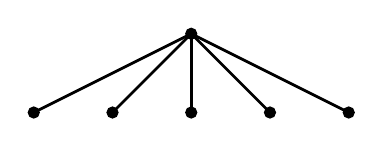
\begin{tikzpicture}
			\draw [fill=black] (0,0) circle (2pt);
			\draw [fill=black] (1,0) circle (2pt);
			\draw [fill=black] (2,0) circle (2pt);
			\draw [fill=black] (3,0) circle (2pt);
			\draw [fill=black] (4,0) circle (2pt);
			\draw [fill=black] (2,1) circle (2pt);
			\draw [line width=1pt] (0,0)-- (2,1);
			\draw [line width=1pt] (1,0)-- (2,1);
			\draw [line width=1pt] (2,0)-- (2,1);
			\draw [line width=1pt] (3,0)-- (2,1);
			\draw [line width=1pt] (4,0)-- (2,1);
		\end{tikzpicture} & 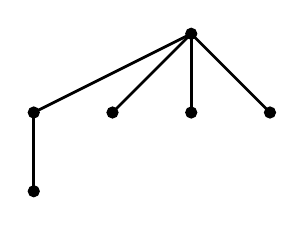
\begin{tikzpicture}
			\draw [fill=black] (0,0) circle (2pt);
			\draw [fill=black] (1,0) circle (2pt);
			\draw [fill=black] (2,0) circle (2pt);
			\draw [fill=black] (3,0) circle (2pt);
			\draw [fill=black] (0,-1) circle (2pt);
			\draw [fill=black] (2,1) circle (2pt);
			\draw [line width=1pt] (0,0)-- (2,1);
			\draw [line width=1pt] (1,0)-- (2,1);
			\draw [line width=1pt] (2,0)-- (2,1);
			\draw [line width=1pt] (3,0)-- (2,1);
			\draw [line width=1pt] (0,0)-- (0,-1);
		\end{tikzpicture} &  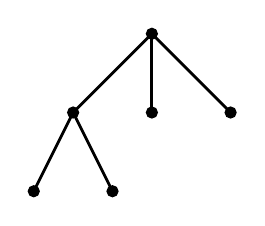
\begin{tikzpicture}
			\draw [fill=black] (1,0) circle (2pt);
			\draw [fill=black] (2,0) circle (2pt);
			\draw [fill=black] (3,0) circle (2pt);
			\draw [fill=black] (0.5,-1) circle (2pt);
			\draw [fill=black] (1.5,-1) circle (2pt);
			\draw [fill=black] (2,1) circle (2pt);
			\draw [line width=1pt] (1,0)-- (2,1);
			\draw [line width=1pt] (2,0)-- (2,1);
			\draw [line width=1pt] (3,0)-- (2,1);
			\draw [line width=1pt] (1,0)-- (0.5,-1);
			\draw [line width=1pt] (1,0)-- (1.5,-1);
		\end{tikzpicture}  \tabularnewline
			$(5,1,1,1,1,1)$ & $(4,2,1,1,1,1)$ & $(3,3,1,1,1,1)$
	\end{tabular}
	
	
	\begin{tabular}{cc}
		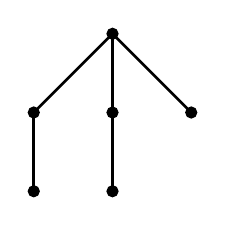
\begin{tikzpicture}
			\draw [fill=black] (1,0) circle (2pt);
			\draw [fill=black] (2,0) circle (2pt);
			\draw [fill=black] (3,0) circle (2pt);
			\draw [fill=black] (1,-1) circle (2pt);
			\draw [fill=black] (2,-1) circle (2pt);
			\draw [fill=black] (2,1) circle (2pt);
			\draw [line width=1pt] (1,0)-- (2,1);
			\draw [line width=1pt] (2,0)-- (2,1);
			\draw [line width=1pt] (3,0)-- (2,1);
			\draw [line width=1pt] (1,0)-- (1,-1);
			\draw [line width=1pt] (2,0)-- (2,-1);
		\end{tikzpicture} \hspace{1cm} 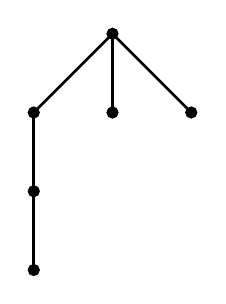
\begin{tikzpicture}
			\draw [fill=black] (1,0) circle (2pt);
			\draw [fill=black] (2,0) circle (2pt);
			\draw [fill=black] (3,0) circle (2pt);
			\draw [fill=black] (1,-1) circle (2pt);
			\draw [fill=black] (1,-2) circle (2pt);
			\draw [fill=black] (2,1) circle (2pt);
			\draw [line width=1pt] (1,0)-- (2,1);
			\draw [line width=1pt] (2,0)-- (2,1);
			\draw [line width=1pt] (3,0)-- (2,1);
			\draw [line width=1pt] (1,0)-- (1,-1);
			\draw [line width=1pt] (1,-1)-- (1,-2);
		\end{tikzpicture} & 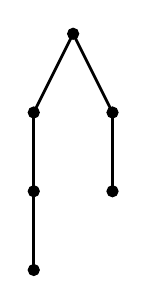
\begin{tikzpicture}
			\draw [fill=black] (1,0) circle (2pt);
			\draw [fill=black] (2,0) circle (2pt);
			\draw [fill=black] (1,-1) circle (2pt);
			\draw [fill=black] (1,-2) circle (2pt);
			\draw [fill=black] (2,-1) circle (2pt);
			\draw [fill=black] (1.5,1) circle (2pt);
			\draw [line width=1pt] (1,0)-- (1.5,1);
			\draw [line width=1pt] (2,0)-- (1.5,1);
			\draw [line width=1pt] (1,0)-- (1,-1);
			\draw [line width=1pt] (1,-1)-- (1,-2);
			\draw [line width=1pt] (2,0)-- (2,-1);
		\end{tikzpicture} \tabularnewline
		$(3,2,2,1,1,1)$ & $(2,2,2,2,1,1)$
	\end{tabular}
}
\end{center}

Összesítés: az $6$ csúcsú fáknak $6$ féle alakja létezik.
\end{solution}
\begin{problem}
Igazoljuk, hogy tetszőleges $n$ esetén azon partíciók száma, melyek
konjugáltja önmaga, megegyezik a csak páratlan, egymástól különböző
számokból álló partíciók számával! 
\end{problem}
\begin{solution}
Adjunk példát olyan partíciókra, melynek a konjugáltja önmaga:

\vspace{0.1cm}
\begin{center}
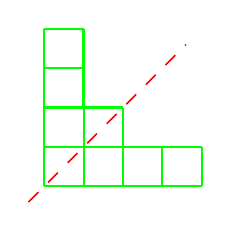
\begin{tikzpicture}
                \draw[step=0.5cm, green, thick] (0,1) grid (0.5,2);
                \draw[step=0.5cm, green, thick] (0,0.5) grid (1,1);
                \draw[step=0.5cm, green, thick] (0,0) grid (2,0.5);
                 \draw [line width=0.6pt,red,dash pattern=on 5pt off 5pt] (-0.2,-0.2)-- (1.8,1.8);
            \end{tikzpicture} \hspace{0.7cm} 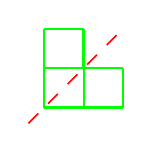
\begin{tikzpicture}
                \draw[step=0.5cm, green, thick] (0,0.5) grid (0.5,1);
                \draw[step=0.5cm, green, thick] (0,0) grid (1,0.5);
                 \draw [line width=0.6pt,red,dash pattern=on 5pt off 5pt] (-0.2,-0.2)-- (1,1);
            \end{tikzpicture} \hspace{0.7cm} 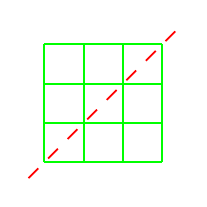
\begin{tikzpicture}
                \draw[step=0.5cm, green, thick] (0,0) grid (1.5,1.5);
                 \draw [line width=0.6pt,red,dash pattern=on 5pt off 5pt] (-0.2,-0.2)-- (1.7,1.7);
            \end{tikzpicture}
\par\end{center}
\begin{center}
$(4,2,1,1)$ \hspace{1.4cm} $(2,1)$ \hspace{1.15cm} $(3,3,3,)$
\par\end{center}
\hspace{0cm}

Észrevehetjük, hogy ezek az első szögfelezőre szimmetrikus partíciók
lesznek. A továbbiakban szimmetrikus partícióknak nevezzük őket.

Most pedig adjunk példát olyan partíciókra is, melyek csak páratlan
és különböző számokból állnak:

\vspace{0.2cm}
\begin{center}
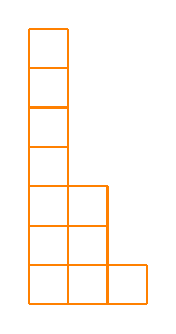
\begin{tikzpicture}
                \draw[step=0.5cm, orange, thick] (0,1.5) grid (0.5,3.5);
                \draw[step=0.5cm, orange, thick] (0,0.5) grid (1,1.5);
                \draw[step=0.5cm, orange, thick] (0,0) grid (1.5,0.5);
            \end{tikzpicture} \hspace{1cm} 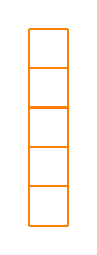
\begin{tikzpicture}
                \draw[step=0.5cm, orange, thick] (0,0) grid (0.5,2.5);
            \end{tikzpicture} \hspace{1cm} 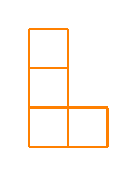
\begin{tikzpicture}
                \draw[step=0.5cm, orange, thick] (0,0.5) grid (0.5,1.5);
                \draw[step=0.5cm, orange, thick] (0,0) grid (1,0.5);
            \end{tikzpicture}
\par\end{center}
\begin{center}
\hspace{0.05cm} $(7,3,1)$ \hspace{1.25cm} $(5)$ \hspace{1.1cm}
$(3,1)$
\par\end{center}
Vizsgáljuk meg, hogy $n=8$ esetén a kétféle partíció száma megegyezik-e.
A megfelelő partíciók az alábbiak:
\begin{center}
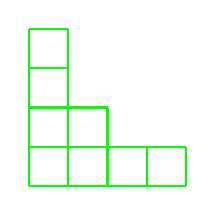
\begin{tikzpicture}
                \draw[step=0.5cm, green, thick] (0,1) grid (0.5,2);
                \draw[step=0.5cm, green, thick] (0,0.5) grid (1,1);
                \draw[step=0.5cm, green, thick] (0,0) grid (2,0.5);
            \end{tikzpicture} \hspace{0.5cm} 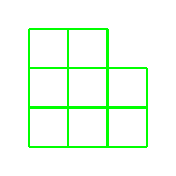
\begin{tikzpicture}
                \draw[step=0.5cm, green, thick] (0,1) grid (1,1.5);
                \draw[step=0.5cm, green, thick] (0,0) grid (1.5,1);
            \end{tikzpicture} \hspace{1cm} 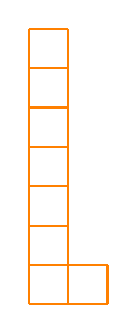
\begin{tikzpicture}
                \draw[step=0.5cm, orange, thick] (0,0.5) grid (0.5,3.5);
                \draw[step=0.5cm, orange, thick] (0,0) grid (1,0.5);
            \end{tikzpicture} \hspace{0.5cm} 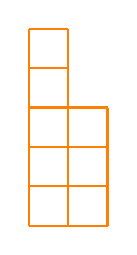
\begin{tikzpicture}
                \draw[step=0.5cm, orange, thick] (0,1.5) grid (0.5,2.5);
                \draw[step=0.5cm, orange, thick] (0,0) grid (1,1.5);
            \end{tikzpicture}
\par\end{center}
\begin{center}
\hspace{0.1cm} $(4,2,1,1)$ \hspace{0.9cm} $(3,3,2)$ \hspace{1.4cm}
$(7,1)$ \hspace{0.75cm} $(5,3)$
\par\end{center}
\begin{center}
\vspace{0.4cm}
\par\end{center}
Valóban megállapítható, hogy a két féle partíció száma megegyezik
egymással, hiszen mindkettőből kettő van. A továbbiakban kapcsolatot
kell keresnünk ezek között, vegyük észre az alábbi leképezést:

\vspace{0.2cm}

\hspace{0.1cm} 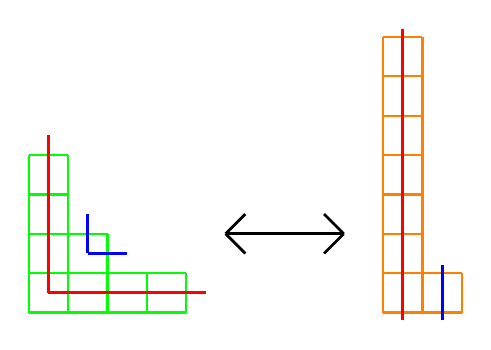
\begin{tikzpicture}
                \draw[step=0.5cm, green, thick] (0,1) grid (0.5,2);
                \draw[step=0.5cm, green, thick] (0,0.5) grid (1,1);
                \draw[step=0.5cm, green, thick] (0,0) grid (2,0.5);
                \draw [line width=1pt,red] (0.25,0.25)-- (0.25,2.25);
                \draw [line width=1pt,red] (0.25,0.25)-- (2.25,0.25);
                \draw [line width=1pt,blue] (0.75,0.75)-- (0.75,1.25);
                \draw [line width=1pt,blue] (0.75,0.75)-- (1.25,0.75);
                \draw [line width=1pt,black] (2.5,1)-- (4,1);
                \draw [line width=1pt,black] (2.5,1)-- (2.75,1.25);
                \draw [line width=1pt,black] (2.5,1)-- (2.75,0.75);
                \draw [line width=1pt,black] (4,1)-- (3.75,0.75);
                \draw [line width=1pt,black] (4,1)-- (3.75,1.25);
                \draw[step=0.5cm, orange, thick] (4.5,0) grid (5.5,0.5);
                \draw[step=0.5cm, orange, thick] (4.5,0.5) grid (5,3.5);
                \draw [line width=1pt,orange] (4.5,0)-- (4.5,3.5);
                \draw [line width=1pt,red] (4.75,-0.1)-- (4.75,3.6);
                \draw [line width=1pt,blue] (5.25,-0.1)-- (5.25,0.6);
            \end{tikzpicture} \hspace{0.5cm} 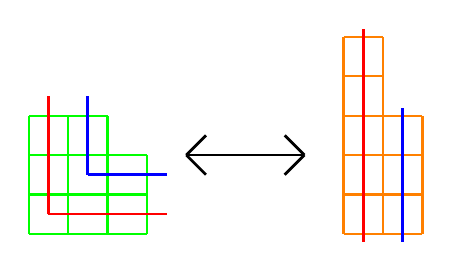
\begin{tikzpicture}
                \draw[step=0.5cm, green, thick] (0,1) grid (1,1.5);
                \draw[step=0.5cm, green, thick] (0,0) grid (1.5,1);
                \draw [line width=1pt,red] (0.25,0.25)-- (0.25,1.75);
                \draw [line width=1pt,red] (0.25,0.25)-- (1.75,0.25);
                \draw [line width=1pt,blue] (0.75,0.75)-- (0.75,1.75);
                \draw [line width=1pt,blue] (0.75,0.75)-- (1.75,0.75);
                \draw [line width=1pt,black] (2,1)-- (3.5,1);
                \draw [line width=1pt,black] (2,1)-- (2.25,1.25);
                \draw [line width=1pt,black] (2,1)-- (2.25,0.75);
                \draw [line width=1pt,black] (3.5,1)-- (3.25,0.75);
                \draw [line width=1pt,black] (3.5,1)-- (3.25,1.25);
                \draw[step=0.5cm, orange, thick] (4,1.5) grid (4.5,2.5);
                \draw[step=0.5cm, orange, thick] (4,0) grid (5,1.5);
                \draw [line width=1pt,orange] (4,0)-- (4,2.5);
                \draw [line width=1pt,red] (4.25,-0.1)-- (4.25,2.6);
                \draw [line width=1pt,blue] (4.75,-0.1)-- (4.75,1.6);
            \end{tikzpicture}

\hspace{0.4cm} $(4,2,1,1)$ \hspace{2.65cm} $(7,1)$ \hspace{0.8cm}
$(3,3,2)$ \hspace{2.6cm} $(5,3)$

\vspace{0.4cm}

Ez a leképezés általános $n$ esetén is hasonlóan elvégezhető. Ha
a szimmetrikus partíciókból indulunk ki, akkor biztos át tudjuk írni
őket csak páratlan számok összegére, mert a főátlóról kiindulva felfele
és jobbra ugyanannyi négyzet van, vagyis a főátlón lévővel együtt
páratlan számú. Ezáltal páratlan számú partícióra tudjuk felírni a
szimmetrikus partíciókat és azért lesznek ezek a számok különbözőek
is, mert ahogy haladunk felfele a főátlón úgy az oszlopok magassága
sem növekedhet, hiszen a partíciókban csökkenő sorrendben vannak a
számok. Ezáltal az átírt páratlan számok is csökkenő sorrendben lesznek.
Ha a különböző páratlan számokból felírt partíciókból indulunk ki,
akkor szintén megkaphatjuk a szimmetrikusakat, ha minden oszlopot
a középső négyzetnél betűrünk. Mivel egyértelműen megfeleltethető
egymásnak a két halmaz, ezért ugyanannyi elemmel rendelkeznek. 
\end{solution}

\section*{Házi feladatok}
\begin{problem}
Írjuk fel az alábbi partíciókat: 
\begin{enumerate}
\item[a)] $p(6)$; 
\item[b)] $p(10,4)$; 
\item[c)] $q(12,5)$; 
\item[d)] $s(11,4,5)$. 
\end{enumerate}
\end{problem}
\begin{solution}
\hspace{0cm}
\begin{enumerate}
\item[a)] $p(6)=11$, a lehetséges partíciók:

\begin{minipage}[c]{0.3\textwidth}%
 \hspace{0cm} 
\begin{itemize}
\item[] 6 
\item[] 5 + 1 
\item[] 4 + 2 
\item[] 4 + 1 + 1 
\item[] 3 + 3 
\item[] 3 + 2 + 1 
\end{itemize}
\hspace{0cm} %
\end{minipage}%
\begin{minipage}[c]{0.45\textwidth}%
 \hspace{0cm} 
\begin{itemize}
\item[] 3 + 1 + 1 + 1 
\item[] 2 + 2 + 2 
\item[] 2 + 2 + 1 + 1 
\item[] 2 + 1 + 1 + 1 + 1 
\item[] 1 + 1 + 1 + 1 + 1 + 1 
\end{itemize}
\hspace{0cm} %
\end{minipage}
\item[b)] $p(10,4)=9$, a lehetséges partíciók:

\begin{minipage}[c]{0.3\textwidth}%
 \hspace{0cm} 
\begin{itemize}
\item[] 7 + 1 + 1 + 1 
\item[] 6 + 2 + 1 + 1 
\item[] 5 + 3 + 1 + 1 
\item[] 5 + 2 + 2 + 1 
\end{itemize}
\hspace{0cm} %
\end{minipage}%
\begin{minipage}[c]{0.45\textwidth}%
 \hspace{0cm} 
\begin{itemize}
\item[] 4 + 4 + 1 + 1 
\item[] 4 + 3 + 2 + 1 
\item[] 4 + 2 + 2 + 2 
\item[] 3 + 3 + 3 + 1 
\item[] 3 + 3 + 2 + 2 
\end{itemize}
\hspace{0cm} %
\end{minipage}
\item[c)] $q(12,5)=13$, a lehetséges partíciók:

\begin{minipage}[c]{0.34\textwidth}%
 \hspace{0cm} 
\begin{itemize}
\item[] 5 + 5 + 2 
\item[] 5 + 5 + 1 + 1 
\item[] 5 + 4 + 3 
\item[] 5 + 4 + 2 + 1 
\item[] 5 + 4 + 1 + 1 + 1 
\item[] 5 + 3 + 3 + 1 
\item[] 5 + 3 + 2 + 2 
\end{itemize}
\hspace{0cm} %
\end{minipage}%
\begin{minipage}[c]{0.49\textwidth}%
 \hspace{0cm} 
\begin{itemize}
\item[] 5 + 3 + 2 + 1 + 1 
\item[] 5 + 3 + 1 + 1 + 1 + 1 
\item[] 5 + 2 + 2 + 2 + 1 
\item[] 5 + 2 + 2 + 1 + 1 + 1 
\item[] 5 + 2 + 1 + 1 + 1 + 1 + 1 
\item[] 5 + 1 + 1 + 1 + 1 + 1 + 1 + 1 
\end{itemize}
\hspace{0cm} %
\end{minipage}
\item[d)] $s(11,4,5)=6$, a lehetséges partíciók:

\begin{minipage}[c]{0.34\textwidth}%
 \hspace{0cm} 
\begin{itemize}
\item[] 4 + 4 + 1 + 1 + 1 
\item[] 4 + 3 + 2 + 1 + 1 
\item[] 4 + 2 + 2 + 2 + 1 
\end{itemize}
\hspace{0cm} %
\end{minipage}%
\begin{minipage}[c]{0.49\textwidth}%
 \hspace{0cm} 
\begin{itemize}
\item[] 3 + 3 + 3 + 1 + 1 
\item[] 3 + 3 + 2 + 2 + 1 
\item[] 3 + 2 + 2 + 2 + 2 
\end{itemize}
\hspace{0cm} %
\end{minipage}

\end{enumerate}
\end{solution}
\begin{problem}
Rajzoljuk fel azokat a $7$ csúccsal rendelkező fákat, melyek maximális
fokszáma nagyobb vagy egyenlő, mint $4$! 
\end{problem}
\begin{solution}
A 7 csúcsú fáknak 6 élük van és a csúcsok fokszámának összege 12.
Feladatunk a 12 azon partícióit meghatározni melyeknek legnagyobb
elem legalább 4 és legfentebb 6, valamint pontosan 7 szám összegéből
áll. Ezek a következőek:

\hspace{0cm}

\hspace{0.3cm} (6,1,1,1,1,1,1) \hspace{0.5cm} (5,2,1,1,1,1,1) \hspace{0.5cm}
(4,3,1,1,1,1,1) \hspace{0.5cm} (4,2,2,1,1,1,1)

\hspace{0cm}

A továbbiakban azt kell megvizsgálnunk, hogy ezekkel a partíciókkal
milyen ábrák készíthetőek el.

\begin{center}
{\setlength{\tabcolsep}{18pt}
	\begin{tabular}{cc}
		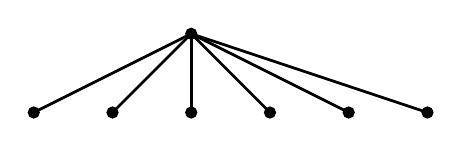
\begin{tikzpicture}
			\draw [fill=black] (0,0) circle (2pt);
			\draw [fill=black] (1,0) circle (2pt);
			\draw [fill=black] (2,0) circle (2pt);
			\draw [fill=black] (3,0) circle (2pt);
			\draw [fill=black] (4,0) circle (2pt);
			\draw [fill=black] (2,1) circle (2pt);
			\draw [fill=black] (5,0) circle (2pt);
			\draw [line width=1pt] (0,0)-- (2,1);
			\draw [line width=1pt] (1,0)-- (2,1);
			\draw [line width=1pt] (2,0)-- (2,1);
			\draw [line width=1pt] (3,0)-- (2,1);
			\draw [line width=1pt] (4,0)-- (2,1);
			\draw [line width=1pt] (5,0)-- (2,1);
		\end{tikzpicture} & 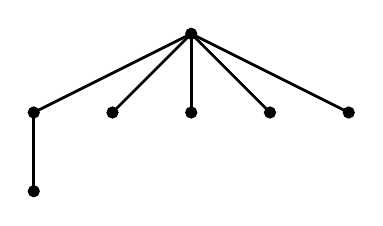
\begin{tikzpicture}
			\draw [fill=black] (0,0) circle (2pt);
			\draw [fill=black] (1,0) circle (2pt);
			\draw [fill=black] (2,0) circle (2pt);
			\draw [fill=black] (3,0) circle (2pt);
			\draw [fill=black] (4,0) circle (2pt);
			\draw [fill=black] (2,1) circle (2pt);
			\draw [fill=black] (0,-1) circle (2pt);
			\draw [line width=1pt] (0,0)-- (2,1);
			\draw [line width=1pt] (1,0)-- (2,1);
			\draw [line width=1pt] (2,0)-- (2,1);
			\draw [line width=1pt] (3,0)-- (2,1);
			\draw [line width=1pt] (4,0)-- (2,1);
			\draw [line width=1pt] (0,0)-- (0,-1);
		\end{tikzpicture} \tabularnewline
		$(6,1,1,1,1,1,1)$ & $(5,2,1,1,1,1,1)$
	\end{tabular}
	\begin{tabular}{ccc}
		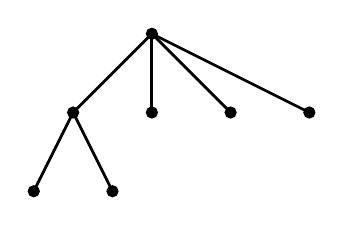
\begin{tikzpicture}
			\draw [fill=black] (1,0) circle (2pt);
			\draw [fill=black] (2,0) circle (2pt);
			\draw [fill=black] (3,0) circle (2pt);
			\draw [fill=black] (4,0) circle (2pt);
			\draw [fill=black] (2,1) circle (2pt);
			\draw [fill=black] (0.5,-1) circle (2pt);
			\draw [fill=black] (1.5,-1) circle (2pt);
			\draw [line width=1pt] (1,0)-- (2,1);
			\draw [line width=1pt] (2,0)-- (2,1);
			\draw [line width=1pt] (3,0)-- (2,1);
			\draw [line width=1pt] (4,0)-- (2,1);
			\draw [line width=1pt] (1,0)-- (0.5,-1);
			\draw [line width=1pt] (1,0)-- (1.5,-1);
		\end{tikzpicture} & \begin{tikzpicture}
			\draw [fill=black] (1,0) circle (2pt);
			\draw [fill=black] (2,0) circle (2pt);
			\draw [fill=black] (3,0) circle (2pt);
			\draw [fill=black] (4,0) circle (2pt);
			\draw [fill=black] (2,1) circle (2pt);
			\draw [fill=black] (1,-1) circle (2pt);
			\draw [fill=black] (2,-1) circle (2pt);
			\draw [line width=1pt] (1,0)-- (2,1);
			\draw [line width=1pt] (2,0)-- (2,1);
			\draw [line width=1pt] (3,0)-- (2,1);
			\draw [line width=1pt] (4,0)-- (2,1);
			\draw [line width=1pt] (1,0)-- (1,-1);
			\draw [line width=1pt] (2,0)-- (2,-1);
		\end{tikzpicture} \hspace{0.5cm} \begin{tikzpicture}
			\draw [fill=black] (1,0) circle (2pt);
			\draw [fill=black] (2,0) circle (2pt);
			\draw [fill=black] (3,0) circle (2pt);
			\draw [fill=black] (4,0) circle (2pt);
			\draw [fill=black] (2,1) circle (2pt);
			\draw [fill=black] (1,-1) circle (2pt);
			\draw [fill=black] (1,-2) circle (2pt);
			\draw [line width=1pt] (1,0)-- (2,1);
			\draw [line width=1pt] (2,0)-- (2,1);
			\draw [line width=1pt] (3,0)-- (2,1);
			\draw [line width=1pt] (4,0)-- (2,1);
			\draw [line width=1pt] (1,0)-- (1,-1);
			\draw [line width=1pt] (1,-1)-- (1,-2);
		\end{tikzpicture} \tabularnewline
		$(4,3,1,1,1,1,1)$ & $(4,2,2,1,1,1,1)$
	\end{tabular}
}
\end{center}

Tehát 5 féle fát lehet felrajzolni úgy, hogy azok teljesítsék a feladat
feltételeit. 
\end{solution}
\begin{problem}
Hány olyan egymáshoz nem hasonló háromszög van, amely tompaszögű,
továbbá nem egyenlő szárú és mindegyik szöge fokokban mérve egész
számot ad? 
\end{problem}
\begin{solution}
Ha tompaszögű egy háromszög, akkor egyik szöge $90^{\circ}$-nál nagyobb
és kisebb, mint $180^{\circ}$. Mivel ki van kötve, hogy nem egyenlő
szárú, ezért a tompaszög $91^{\circ}$ és $177^{\circ}$ között változik.
Ekkor a másik két szög összege $89^{\circ}$ és $3^{\circ}$ közötti
értékeket vehet fel. Tulajdonképpen $p(k,2)$-t kell meghatároznunk
minden $3\leq k\leq89$ esetén úgy, hogy a páros számok esetén levonjuk
azt az egy esetet, amikor amikor a két szög egyenlő. Így a következő
összegzést kapjuk: 
\[
1+1+2+2+3+3+\dots+42+43+43+44=2\cdot\frac{44\cdot43}{2}+44=44\cdot43+44=44^{2}=1936.
\]
\end{solution}
\begin{problem}
Határozzuk meg $p(n,1)$ és $p(n,2)$ értékét az $n$ függvényében! 
\end{problem}
\begin{solution}
Először is $p(n,1)=1$, mert minden szám csak saját magával írható
fel 1 szám felbontásaként. Továbbá vizsgáljuk meg, hogy $p(n,2)$
milyen értékek vesz fel az szerint, hogy $n$ páros vagy páratlan.

Ha $n$ páros, vagyis $n=2k$, akkor $k$ féleképpen írható fel két
szám összegeként, mert ezek a partíciók $(i,n-i)$ alakúak, ahol $1\leq i\leq k$.

Ha $n$ páratlan, vagyis $n=2k+1$ alakú, akkor is $k$ féleképpen
írható fel két szám összegeként, mert ebben az esetben a partíciók
szintén $(i,n-i)$ alakúak, ahol $1\leq i\leq k$.

A két eset egyesíthető, ha egészrészt használunk, hiszen $p(n,2)=\left[\frac{n}{2}\right]=k$
mindkét esetben. 
\end{solution}
\begin{problem}
Azokat a természetes számokat, amelyek felírhatóak két vagy több egymás
utáni pozitív egész szám összegeként udvarias számoknak nevezzük.
Az udvariasságnak van mértéke is: egy szám udvariasságának annyi a
mértéke ahányféleképpen fel lehet írni ilyen összegként. 
\begin{enumerate}
\item[a)] A páratlan számok udvariasak? 
\item[b)] Adjunk három példát nem udvarias számra! 
\item[c)] Adjunk egy-egy példát 2 és 3 mértékű udvarias számra! 
\end{enumerate}
\end{problem}
\begin{solution}
\hspace{0cm}
\begin{enumerate}
\item[a)] Igen, az 1-nél nagyobb páratlan számok mindig udvariasak, mert egy
páratlan szám általános alakja $2k+1$, $k>0$ és $2k+1=k+(k+1)$,
vagyis mindig felírható két egymás utáni természetes szám összegeként. 
\item[b)] Rövid próbálgatás után megsejthetjük, hogy a 2 hatványait nem tudjuk
ilyen összegként felírni, ezért ha csak három példát kell megadnunk
az lehet az 1,2,4. 
\item[c)] Vegyünk először két mértékű udvarias számot. Erre példa lehet a 9,
hiszen $9=4+5=2+3+4$. Ugyanakkor három mértékű udvarias számnak megadhatjuk
a 15-öt, hiszen $15=7+8=4+5+6=1+2+3+4+5$. 
\end{enumerate}
\end{solution}
\begin{problem}
Tetszőleges $n,k\in\mathbb{N}$, $k\leq n$ esetén igazoljuk, hogy:
\[
p(n,1)+p(n,2)+...+p(n,k)=p(n+k,k).
\]
\end{problem}
\begin{solution}
Abból indulunk ki, hogy egy olyan összegnél, amikor az $n+k$-t bontjuk
fel $k$ részre a felbontás mindegyik tagja legalább 1. Ha minden
oszlopból levennénk 1 értéket, akkor ezeknek a partícióknak a száma
ugyanaz maradna, mint a $p(n+k,k)$, hiszen egyik új partíció se lehetne
megegyező, mivel különbözőekből indultunk ki. Vizsgáljuk meg az innen
kapott partíciókat. Amit biztosan állíthatunk, hogy $n$ valamely
partícióit kaptuk meg, hiszen $n+k-k=n$. Ugyanakkor attól függően,
hogy az eredeti partíciókban hány 1-es volt meg tudjuk mondani, hogy
a mostani felosztások milyen félék, hány oszlopból állnak. Mivel az
$n+k$ partícióiban lehetett $0,1,2,\dots,k-1$ darab 1-es, ezért
miután $k$ értéket elvettünk a kapott $n$ partícióit is $k$ csoportba
sorolhatjuk az szerint, hogy $k,k-1,\dots,2,1$ oszlopa van. De akkor
ilyen meggondolásból a partíciók száma pont a $p(n,k)+\dots+p(n,2)+p(n,1)$
összeget fogja jelenteni. Tehát valóban igaz $n,k\in\mathbb{N}$,
$k\leq n$ esetén, hogy 
\[
p(n,1)+p(n,2)+...+p(n,k)=p(n+k,k).
\]
\end{solution}

\section*{Nehezebb feladatok}
\begin{extraproblem}[Csurka-Molnár Hanna]
Határozzuk meg $p(n,3)$ értékét $n$ függvényében! 
\end{extraproblem}
\begin{solution}
$3$ oszlopból álló Young-diagramokat kell előállítanunk $n$ kis
négyzetből. Először számoljuk meg azon diagramok számát, ahol az oszlopok
nem feltétlenül magasság szerinti csökkenő sorrendben követik egymást.
Ehhez egy $100$ négyzetből álló oszlopot kétszer kell bárhol elszelnünk
(a vágások előtt, között és után is kell lennie legalább 1 négyzetnek),
majd az első vágás előtti, a két vágás közötti és a második vágás
utáni négyzeteket helyezzük a három oszlopba. Ez $C_{n-1}^{2}=\frac{(n-1)!}{2!(n-3)!}=\frac{(n-1)(n-2)}{2}$
módon tehető meg.

Az előző felbontásban többször is szerepelnek partíciók, mivel az
$n=\lambda_{1}+\lambda_{2}+\lambda_{3}$ előállításban figyelmen kívül
hagytuk a $\lambda_{1}\ge\lambda_{2}\ge\lambda_{3}$ megkötést. Ezért
azok a partíciók, ahol $\lambda_{1}>\lambda_{2}>\lambda_{3}$, $3!=6$-szor
voltak számolva. Ezeknek a partícióknak a számát jelöljük $x$-el.
Továbbá, azok a partíciók, ahol $\lambda_{1}=\lambda_{2}>\lambda_{3}$,
vagy $\lambda_{1}>\lambda_{2}=\lambda_{3}$, $C_{3}^{1}=3$-szor voltak
számolva. Ezeknek a partícióknak a számát jelöljük $y$-nal. Amennyiben
$3|n$, megjelenik a $\lambda_{1}=\lambda_{2}=\lambda_{3}$ particionálás,
viszont ez nem ismétlődik. Jelöljük ennek a partíciónak a számát $z$-vel.
$z=1$, ha $3|n$, különben $z=0$. Másként $z=1-\lceil\{\frac{n}{3}\}\rceil$.

Ezek alapján írhatjuk a következő összefüggést: 
\begin{equation}
6x+3y+z=\frac{(n-1)(n-2)}{2}\;.\label{eq:ismetelt_megszamlalas}
\end{equation}

Számoljuk meg $y$-t! Írjuk fel $n$ számot két egyforma és egy különböző
szám összegeként: $n=2a+b$. Ekkor $b$ paritása megegyezik $n$ paritásával.
Ugyanakkor $1\le a\Rightarrow b\le n-2$ és $0<b$. $y$ értékét $b$
lehetséges értékeinek a száma adja meg. Amennyiben $n$ páros, $b\in\{2,4,\dots,n-2\}\Rightarrow y=\frac{n-2}{2}$.
Ha $n$ páratlan, $b\in\{1,3,\dots,n-2\}\Rightarrow y=\frac{n-1}{2}$.
Másként $y=\left\lfloor \frac{n-1}{2}\right\rfloor $.

Kifejezve $x$-et \ref{eq:ismetelt_megszamlalas} egyenletből kapjuk,
hogy: 
\[
x=\frac{1}{6}\left(\frac{(n-1)(n-2)}{2}-3\left\lfloor \frac{n-1}{2}\right\rfloor -\left(1-\left\lceil \left\{ \frac{n}{3}\right\} \right\rceil \right)\right)
\]

A keresett érték pedig 
\begin{align*}
p(n,3) & =x+y+z\\
 & =\frac{1}{6}\left(\frac{(n-1)(n-2)}{2}-3\left\lfloor \frac{n-1}{2}\right\rfloor -\left(1-\left\lceil \left\{ \frac{n}{3}\right\} \right\rceil \right)\right)+\left\lfloor \frac{n-1}{2}\right\rfloor +\left(1-\left\lceil \left\{ \frac{n}{3}\right\} \right\rceil \right)\\
 & =\frac{1}{6}\left(\frac{(n-1)(n-2)}{2}+3\left\lfloor \frac{n-1}{2}\right\rfloor +5\left(1-\left\lceil \left\{ \frac{n}{3}\right\} \right\rceil \right)\right)
\end{align*}
\end{solution}
\begin{extraproblem}[Czofa Vivien]
Hányféleképpen lehet a 20-at három különböző pozitív egész szám összegeként
felírni, ha a sorrend nem számít?
\end{extraproblem}
\bigskip{}

\begin{solution}
Keressük azokat a hármasokat $(a,b,c)$, ahol $a<b<c$ és $a+b+c=20$.

Mivel $a<b<c$, ezért $a\geq1$, $b\geq a+1$, $c\geq b+1$.

Összeadva: $a+(a+1)+(a+2)=3a+3\leq20$, így $a\leq5$.

Vizsgáljuk az összes lehetséges $a$ értéket:

$a=1$: $(1,2,17),(1,3,16),(1,4,15),(1,5,14),(1,6,13),(1,7,12),(1,8,11)$
--- összesen 7 lehetőség.

$a=2$: $(2,3,15),(2,4,14),(2,5,13),(2,6,12),(2,7,11),(2,8,10)$ ---
összesen 6 lehetőség.

$a=3$: $(3,4,13),(3,5,12),(3,6,11),(3,7,10),(3,8,9)$ --- összesen
5 lehetőség.

$a=4$: $(4,5,11),(4,6,10),(4,7,9)$ --- összesen 3 lehetőség.

$a=5$: $(5,6,9),(5,7,8)$ --- összesen 2 lehetőség.

\bigskip{}

\textbf{Összesen:} $7+6+5+3+2=23$ különböző partíció.
\end{solution}
\begin{extraproblem}[Czofa Vivien]
Hányféleképpen lehet a 20-at felírni pozitív egész számok összegeként
úgy, hogy minden rész páros szám legyen?
\end{extraproblem}
\bigskip{}

\begin{solution}
Mivel a felírandó szám csak páros részekből állhat, ezért érdemes
a számot kettővel osztani, és így a 20 helyett a 10 számot kell partícionálnunk
tetszőleges pozitív egészek összegeként.

Az eredeti partíció minden tagját meg kétszerezzük, így visszakapjuk
a 20-at páros számok összegeként.

\bigskip{}

\textbf{A 10 összes partíciója:}

$10$

$9+1$

$8+2$

$7+3$

$7+2+1$

$6+4$

$6+3+1$

$6+2+2$

$5+5$

$5+4+1$

$5+3+2$

$5+2+2+1$

$4+4+2$

$4+3+3$

$4+3+2+1$

$4+2+2+2$

$3+3+3+1$

$3+3+2+2$

$3+2+2+2+1$

$2+2+2+2+2$

\bigskip{}

\textbf{Következtetés:}

A 10 számnak összesen 20 partíciója van.

Ez azt jelenti, hogy a 20 számnak pontosan \textbf{20} partíciója
van, ahol minden rész páros szám.
\end{solution}
\begin{extraproblem}[Miklós Dóra]
Igazoljuk, hogy $p(1)+p(2)+\dots+p(n)<p(2n)$ minden $n\geq1$ számra,
ahol $p(n)$ a partíciófüggvény. 
\end{extraproblem}
\begin{solution}
Megoldás 1 Legyen $k=a_{1}+a_{2}+\dots+a_{r}$ egy tetszőleges partíciója
a $k$ számnak $(1\leq k\leq n)$, ahol $k\geq a_{1}\geq a_{2}\geq\dots\geq a_{r}\geq1$.
\\
Akkor 
\[
2n=(2n-k)+a_{1}+a_{2}+\dots+a_{r},
\]
ahol $2n-k\geq n\geq k\geq a_{1}\geq a_{2}\geq\dots\geq a_{r}\geq1$,
és következik, hogy ez egy partíciója $2n$-nek. \\
Így egy olyan megfeleltetést kapunk, amely a $k$ számok $(1\leq k\leq n)$
partícióihoz a $2n$ szám partícióit rendeli hozzá. A $k$ számok
$(1\leq k\leq n)$ különböző partíciói a $2n$ szám különböző partíciói
felelnek meg. Valóban, ha $k_{1}\neq k_{2}$, akkor $2n-k_{1}\neq2n-k_{2}$,
így a $2n$ azon partíciói, amelyekhez $k_{1}$ és $k_{2}$ partíciók
rendelik biztosan különbözők. Ha pedig $k$ rögzített és két különböző
partícióját tekintjük, akkor a megfelelő partíciókban az első tagok
egyenlők, de azt követően legalább egy tag különbözik.

Tehát ez egy injektív megfeleltetés. Ugyanakkor nem szűkítjük, mert
pl. a $2n=2n$ egytagú partíció nem származtatható ilyen módon. Ezzel
igazoltuk az adott egyenlőtlenséget, amely szigorú minden $n\geq1$-re.
Vizsgáljuk részletesen az $n=3$ és $n=4$ eseteket! 
\end{solution}
\begin{extraproblem}[Gál Tamara]
Egy Hargita megyei önkormányzat 10 millió lejes pályázati támogatást
nyert el, amelyet négy különböző település -- \textbf{Csíkszereda},
\textbf{Gyergyószentmiklós}, \textbf{Székelyudvarhely} és \textbf{Tusnádfürdő}
-- között kell szétosztani helyi fejlesztések céljára.

Az elosztásnak a következő feltételeknek kell megfelelnie:
\begin{itemize}
\item Minden település legalább \textbf{1 millió lejt} kap. 
\item Egyik település sem kaphat kétszer annyit, mint bármelyik másik. 
\item Az elosztás során a pénzt egész millió lejekben mérik. 
\end{itemize}
Hányféleképpen lehet a 10 millió lejt az adott feltételek szerint
szétosztani a települések között? 
\end{extraproblem}
\begin{solution}
Tekintsük a 10 természetes szám 4 pozitív egész számra történő partícióit,
vagyis keressük azokat az elosztásokat, ahol:

\[
a+b+c+d=10,\quad a,b,c,d\in\mathbb{N},\quad\text{és }a\leq b\leq c\leq d
\]

Ezután kiszűrjük azokat az elosztásokat, amelyek nem felelnek meg
a következő feltételnek:

\[
\frac{\text{legnagyobb összeg}}{\text{legkisebb összeg}}<2
\]

Végigvizsgálva az összes ilyen partíciót:
\begin{center}
\begin{tabular}{|c|c|c|}
\hline 
\textbf{Partíció} & \textbf{Legnagyobb / legkisebb} & \textbf{Elfogadható?}\tabularnewline
\hline 
(1,1,1,7) & 7 & nem jó\tabularnewline
(1,1,2,6) & 6 & nem jó\tabularnewline
(1,1,3,5) & 5 & nem jó\tabularnewline
(1,1,4,4) & 4 & nem jó\tabularnewline
(1,2,2,5) & 5 & nem jó\tabularnewline
(1,2,3,4) & 4 & nem jó\tabularnewline
(2,2,2,4) & 2 & nem jó\tabularnewline
(2,2,3,3) & 1.5 & jó\tabularnewline
\hline 
\end{tabular}
\par\end{center}
Csak egyetlen partíció felel meg minden feltételnek: $(2,2,3,3)$

Ez azt jelenti, hogy:
\begin{itemize}
\item Csíkszereda kap: 2 millió lejt 
\item Gyergyószentmiklós kap: 2 millió lejt 
\item Székelyudvarhely kap: 3 millió lejt 
\item Tusnádfürdő kap: 3 millió lejt 
\end{itemize}
A megadott feltételek szerint csak egyféleképpen lehet igazságosan
elosztani a 10 millió lejt a négy település között: 
\[
\boxed{(2,2,3,3)}
\]
\end{solution}
\begin{extraproblem}[Gál Tamara]
Jelöljük $p_{4}(n)$-vel azon partíciók számát, amelyekben $n$ felírható
olyan összegek formájában, ahol minden összeadandó tag legalább 4,
és a sorrend nem számít. Határozd meg $p_{4}(20)$-t, azaz hányféleképpen
írható fel 20 olyan természetes számok összegeként, amelyek mindegyike
legalább 4. 
\end{extraproblem}
\begin{solution}
A feladat szerint azt kell meghatározni, hogy hányféleképpen írható
fel 
\[
20=a_{1}+a_{2}+\cdots+a_{k},
\]
ahol minden tag $a_{i}\ge4$ és a sorrend nem számít (tehát a partíciók
rendezett, nem pedig permutációk). Mivel a tagok minimumértéke 4,
az esetleges részek száma $k$ maximuma az, amikor $k\cdot4\le20$,
így $k\le5$.

Az alábbiakban csoportosítva találhatóak a megoldások: \\
\textbf{ 1 tag (k = 1)}\\
 
\begin{enumerate}
[label=(\alph*)]
\item $(20)$ 
\end{enumerate}
\textbf{2 tag (k = 2)}\\
 Keressük az $a+b=20$ megoldásait úgy, hogy $4\le a\le b$: 
\begin{enumerate}
[label=(\alph*)]
\item $(4,\,16)$ 
\item $(5,\,15)$ 
\item $(6,\,14)$ 
\item $(7,\,13)$ 
\item $(8,\,12)$ 
\item $(9,\,11)$ 
\item $(10,\,10)$ 
\end{enumerate}
\textbf{3 tag (k = 3)}\\
 Itt $a+b+c=20$ minden $a,b,c\ge4$ és $a\le b\le c$. A kényelmes
módszer: vonjunk le mindegyikből 4-et, így: 
\[
a'=a-4,\quad b'=b-4,\quad c'=c-4,\quad a'+b'+c'=20-12=8.
\]
Ezután az összes nemcsökkenő megoldás a következő: 
\begin{enumerate}
[label=(\alph*)]
\item $(0,0,8)$ $\to$ $(4,4,12)$ 
\item $(0,1,7)$ $\to$ $(4,5,11)$ 
\item $(0,2,6)$ $\to$ $(4,6,10)$ 
\item $(0,3,5)$ $\to$ $(4,7,9)$ 
\item $(0,4,4)$ $\to$ $(4,8,8)$ 
\item $(1,1,6)$ $\to$ $(5,5,10)$ 
\item $(1,2,5)$ $\to$ $(5,6,9)$ 
\item $(1,3,4)$ $\to$ $(5,7,8)$ 
\item $(2,2,4)$ $\to$ $(6,6,8)$ 
\item $(2,3,3)$ $\to$ $(6,7,7)$ 
\end{enumerate}
\textbf{4 tag (k = 4)}\\
 Ebben az esetben $a+b+c+d=20$ mindegyik tag $\ge4$. Vonjunk le
4-et minden tagból: 
\[
a'+b'+c'+d'=20-16=4.
\]
A nemcsökkenő megoldások a következők: 
\begin{enumerate}
[label=(\alph*)]
\item $(0,0,0,4)$ $\to$ $(4,4,4,8)$ 
\item $(0,0,1,3)$ $\to$ $(4,4,5,7)$ 
\item $(0,0,2,2)$ $\to$ $(4,4,6,6)$ 
\item $(0,1,1,2)$ $\to$ $(4,5,5,6)$ 
\item $(1,1,1,1)$ $\to$ $(5,5,5,5)$ 
\end{enumerate}
\textbf{5 tag (k = 5)}\\
 Itt $a+b+c+d+e=20$ minden tag $\ge4$. Mivel a minimum összeg 5
tag esetén $5\times4=20$, az egyetlen megoldás: 
\begin{enumerate}
\item $(4,\,4,\,4,\,4,\,4)$ 
\end{enumerate}
Összesen a partíciók száma: 
\[
1\,(k=1)+7\,(k=2)+10\,(k=3)+5\,(k=4)+1\,(k=5)=24.
\]
Végleges lista: 
\begin{enumerate}
[label=(\alph*)]
\item $(20)$ 
\item $(4,\,16)$ 
\item $(5,\,15)$ 
\item $(6,\,14)$ 
\item $(7,\,13)$ 
\item $(8,\,12)$ 
\item $(9,\,11)$ 
\item $(10,\,10)$ 
\item $(4,\,4,\,12)$ 
\item $(4,\,5,\,11)$ 
\item $(4,\,6,\,10)$ 
\item $(4,\,7,\,9)$ 
\item $(4,\,8,\,8)$ 
\item $(5,\,5,\,10)$ 
\item $(5,\,6,\,9)$ 
\item $(5,\,7,\,8)$ 
\item $(6,\,6,\,8)$ 
\item $(6,\,7,\,7)$ 
\item $(4,\,4,\,4,\,8)$ 
\item $(4,\,4,\,5,\,7)$ 
\item $(4,\,4,\,6,\,6)$ 
\item $(4,\,5,\,5,\,6)$ 
\item $(5,\,5,\,5,\,5)$ 
\item $(4,\,4,\,4,\,4,\,4)$ 
\end{enumerate}
\end{solution}
\begin{extraproblem}[Gergely Verona]
Legyen $S$ a nemnegatív egész számok halmaza, és jelölje $r_{S}(n)$
a rendezett párok számát $(s_{1},s_{2})$, ahol $s_{1}\in S$, $s_{2}\in S$,
$s_{1}\neq s_{2}$, és $s_{1}+s_{2}=n$. Lehetséges-e úgy felosztani
a nemnegatív egész számokat két halmazra, $A$-ra és $B$-re, hogy
$r_{A}(n)=r_{B}(n)$ minden $n$-re? \emph{(Putnam Mathematical Competition,
2003) }
\end{extraproblem}
\begin{solution}
Definiáljuk $A=\{0,3,5,6,9,\dots\}$-t, mint azon nemnegatív egész
számok halmazát, amelyek a kettes számrendszerben páros számú 1-eseket
tartalmaznak, és definiáljuk $B=\{1,2,4,7,8,\dots\}$-t, mint azon
nemnegatív egész számok halmazát, amelyek a kettes számrendszerben
páratlan számú 1-eseket tartalmaznak.

Definiáljuk $f$ -et, és $g$-t: 
\[
f(x)=\sum_{n\in A}x^{n},\quad g(x)=\sum_{n\in B}x^{n}.
\]

Ekkor:

\[
f(x^{2})+xg(x^{2})=\sum_{n\in A}x^{2n}+\sum_{n\in B}x^{2n+1}=\sum_{2n\in A}x^{2n}+\sum_{2n+1\in A}x^{2n+1}=\sum_{m\in A}x^{m}=f.
\]

Hasonlóan belátható, hogy $g(x^{2})+xf(x^{2})=g.$

Tehát:

\[
f-g=f(x^{2})-g(x^{2})+xg(x^{2})-xf(x^{2})=(1-x)(f(x^{2})-g(x^{2})).
\]

\[
f+g=\sum_{n}x^{n}=\frac{1}{1-x}.
\]

\[
f^{2}-g^{2}=(f-g)(f+g)=f(x^{2})-g(x^{2}).
\]

Másrészről:

\[
f^{2}=\sum_{s\in A,t\in A}x^{s}x^{t}=\sum_{s\in A}x^{2s}+\sum_{s\in A,t\in A,s\neq t}x^{s+t}=f(x^{2})+\sum_{n}r_{A}(n)x^{n}.
\]

Hasonlóan belátható, hogy 
\[
g^{2}=g(x^{2})+\sum_{n}r_{B}(n)x^{n}.
\]

Végül megkapjuk, hogy

\[
\sum_{n}r_{A}(n)x^{n}=f^{2}-f(x^{2})=g^{2}-g(x^{2})=\sum_{n}r_{B}(n)x^{n},
\]

ami bizonyítja, hogy lehetséges a nemnegatív egész számokat két halmazra
felosztani, $A$-ra és $B$-re, úgy, hogy $r_{A}(n)=r_{B}(n)$ minden
$n$-re. 
\end{solution}
\begin{extraproblem}[Kis Aranka-Enikő]
Bizonyítsd be, hogy ha $n$ számtani sorozat $r_{1},r_{2},r_{3},\dots,r_{n}$
rációval a természetes számok egy partícióját alkotják, akkor:
\begin{itemize}
\item[(a)] $r_{1},r_{2},r_{3},\dots,r_{n}$ nem mind különböző. 
\item[(b)] 
\[
\frac{1}{r_{1}}+\frac{1}{r_{2}}+\frac{1}{r_{3}}+\dots+\frac{1}{r_{n}}=1.
\]
\end{itemize}
\end{extraproblem}
\begin{solution}
Jelöljük $a_{j}$-vel ($j=1,\dots,n$) a partíció $j$-edik halmazának
első elemét, és tekintsük az
\[
S_{j}(x)=\sum_{k=0}^{\infty}x^{a_{j}+kr_{j}}
\]
összegeket. Mivel az $(a_{j}+kr_{j})_{k\geq0}$ számtani haladványok
az $N$ egy partícióját alkotják, írhatjuk, hogy

\[
\sum_{j=1}^{n}S_{j}=\sum_{k=0}^{\infty}x^{k}=\frac{1}{1-x}
\]

Tehát

\[
\sum_{j=1}^{n}\frac{x^{a_{j}}}{1-x^{r_{j}}}=\frac{1}{1-x}.
\]
és így 
\[
\sum_{j=1}^{n}\frac{x^{a_{j}}}{1+x+x^{2}+...+x^{r_{j}-1}}=1
\]
Ha $x\to1$, akkor a jobb oldal 1, és a bal oldal és a bal oldal is
az 
\[
\sum_{j=1}^{n}\frac{1}{r_{j}}
\]
-hez tart, tehát 
\[
\sum_{j=1}^{n}\frac{1}{r_{j}}=1.
\]

Ugyanakkor, ha 
\[
r=\max\{r_{j}\mid j=1,2,\dots,n\}
\]
akkor legalább két olyan $j\in\{1,2,\dots,n\}$ érték létezik, amelyre
$r_{j}=r$. Ellenkező esetben, ha $x$ közeledik egy $r$-ed rendű
primitív egységgyökhöz, akkor a jobb oldal $1$ marad, míg a bal oldal
$\infty$-hez tart.
\end{solution}
\begin{extraproblem}[Kiss Andrea-Tímea]
Azokat a természetes számokat, amelyek felírhatóak két vagy több
egymás utáni pozitív egész szám összegeként, udvarias számoknak nevezzük.
Igazoljuk, hogy a $2$ hatványai nem udvarias számok! 
\end{extraproblem}
\begin{solution}
Egy $n$ természetes szám akkor udvarias, ha felírható legalább két
pozitív egész szám összegeként, vagyis létezik $a,k\in\mathbb{N}$,
$a,k\geq1$ úgy, hogy 
\[
n=a+(a+1)+(a+2)+\ldots+(a+k-1),
\]
ahonnan 
\[
n=\dfrac{k\cdot(2a+k-1)}{2}.
\]

Feltételezzük, hogy létezik olyan $m$ természetes szám, amire a $2^{m}$
udvarias szám. Így létezik $a,k\in\mathbb{N}$, $a,k\geq1$ úgy, hogy
\[
2^{m}=\dfrac{k\cdot(2a+k-1)}{2}\Leftrightarrow2^{m-1}=k\cdot(2a+k-1).
\]

Ha $k$ páros, akkor $k-1$ páratlan, így $2a+k-1$ is páratlan. Ha
viszont $k$ páratlan, akkor a $k-1$ páros, így $2a+k-1$ is páros.

Mindkét esetben a $k\cdot(2a+k-1)$ szorzat prímtényezős felbontásában
szerepel egy páratlan szám, így ezen szorzat prímtényezős felbontása
nem állhat csupa $2$-esekből.

Ezek alapján nem létezik olyan kettőhatvány, amely udvarias szám lenne. 
\end{solution}
\begin{extraproblem}[Szabó Kinga]
Felírtam néhány $24$-nél nem nagyobb pozitív egész számot a táblára.
Ezekből bárhogyan választok néhányat (lehet egyet, vagy az összeset
is), azok összegei különbözőek. Legfeljebb hány szám lehet a táblán?
\emph{(Róka Sándor: Válogatás Erdős Pál kedvenc feladataiból) }
\end{extraproblem}
\begin{solution}
$5$ számot könnyű találni, például: $1,2,4,8,16$.

$6$ szám is választható: $11,17,20,22,23,24$.

$8$ szám nem lehet a táblán, mert 8 számból $2^{8}-1=255$ összeget
képezhetünk, ám az összegek értéke legfeljebb

\[
24+23+\ldots+17=164
\]

lehet. Így a skatulyaelv miatt vannak azonos értékű összegek.

$7$ szám sem lehet a táblán. Tegyük fel, hogy mégis. Ha csak a kéttagú
összegek különbözőségét nézzük, akkor két-két különböző szám különbsége
nem lehet azonos. Emiatt a lehető legnagyobb számok:

\[
x,\quad x-1,\quad x-2,\quad x-4,\quad x-7,\quad x-12,\quad x-17
\]

Ezek összege, a legnagyobb összeg még $x=24$-re is kisebb $127$-nél,
azonban $7$ számból $2^{7}-1=127$ összeget képezhetünk, így a skatulyaelv
miatt vannak azonos értékű összegek.
\end{solution}
\begin{extraproblem}[Szabó Kinga]
Az $1,2,\ldots,9$ számokból legfeljebb hány számot lehet kiválasztani,
hogy a páronkénti összegek különbözzenek? (Az összegekben a két tag
különböző.) \emph{(Róka Sándor: Válogatás Erdős Pál kedvenc feladataiból) }
\end{extraproblem}
\begin{solution}
A mohó algoritmussal választhatunk öt számot. Mindig úgy választjuk
a sorozat következő tagját, hogy az első, a legkisebb nem tiltott
számot vesszük: $1,2,3,5,8$.

Ha hat számot választunk, azokból 15 páronkénti összeget képezhetünk,
ám a lehetséges legkisebb összeg $3$, a legnagyobb $17$, így az
összegek 15-féle értéke lehet, tehát mindegyik előáll.

Mivel a $3$ és a $17$ előállítására csak egyetlen lehetőség van:
$3=1+2$, és $17=8+9$, így az $1,2,8$ és $9$ a hat szám között
van. Azonban $1+9=2+8$, tehát hat szám választása esetén nem teljesül,
hogy a páronkénti összegek különbözők. Legfeljebb öt számot választhatunk. 
\end{solution}
\begin{extraproblem}[Száfta Antal]
Egy $n$ természetes szám \emph{különböző részekből álló partíciója}
olyan felbontása, amelyben minden rész különböző és pozitív egész
szám.

Legyen $n=2k+1$ egy tetszőleges páratlan szám.

Bizonyítsd be, hogy a $n$ különböző részekből álló partícióinak száma
megegyezik a $k(k+1)/2$ összeggel, ahol $k$ a legnagyobb olyan szám,
amelyre teljesül, hogy $1+2+\dots+k\leq n$.
\end{extraproblem}
\begin{solution}
Legyen $n=9$. Ekkor $k=4$, mert $1+2+3+4=10>9$, de $1+2+3=6\leq9$.

A tétel szerint tehát a partíciók száma $k(k+1)/2=4\cdot5/2=10$.

\vspace{0.5cm}

\textbf{Bizonyítás:}

Legyen $n=2k+1$ egy rögzített páratlan szám.

Tudjuk, hogy a különböző részekből álló partíciók maximális száma
akkor adódik, ha a lehető legkisebb számokat használjuk: $1,2,3,\dots,k$.

Ezek összege: 
\[
S=1+2+3+\dots+k=\frac{k(k+1)}{2}.
\]

Ez az ún. háromszögszám. Ez a maximális összeg, amit elérhetünk különböző
részekkel, ha legfeljebb $k$ részt használunk.

Mivel $n=2k+1$ páratlan szám, az $n$ nagysága miatt csak $k$ részig
tudunk eljutni úgy, hogy a részek különbözőek maradjanak.

A partíciók száma tehát pontosan megegyezik azzal, ahány módon ki
tudjuk választani a számokat $1,2,\dots,k$ közül úgy, hogy összegük
$n$ legyen.

A klasszikus eredmény (Euler és Ferrers diagramok elmélete) szerint,
ha $n$ páratlan, akkor pontosan $k(k+1)/2$ ilyen partíció létezik.

Ez belátható például azzal, hogy a partíciók megfeleltethetők a háromszögszámok
kiegészítéseinek, mivel $S$ a maximális összeg, és $n$-t ezen összeg
elérésével és a megfelelő részek csökkentésével tudjuk elérni.

\textbf{Következtetés:}

Mivel $n=2k+1$ esetén a partíciók száma pontosan a legnagyobb $k$-ig
tartó sorozat összegével egyezik meg, a feladat állítása igaz.

\[
\boxed{\text{A \ensuremath{n} páratlan szám különböző részekből álló partícióinak száma: }\frac{k(k+1)}{2}.}
\]
\end{solution}
\begin{extraproblem}[Szélyes Klaudia]
Bizonyítsd be, hogy ha $n$ számtani sorozat $r_{1},r_{2},\dots,r_{n}$
rációval a természetes számok egy partícióját alkotják, akkor:
\begin{enumerate}
\item $r_{1},r_{2},\dots,r_{n}$ nem mind különböző, 
\item ${\displaystyle \sum_{j=1}^{n}\frac{1}{r_{j}}=1}$ 
\end{enumerate}
\end{extraproblem}
\bigskip{}

\begin{solution}
Jelöljük $a_{j}$-vel ($1\leq j\leq n$) a partíció $j$-edik halmazának
első elemét, és tekintsük az alábbi sorozatokat:

\[
S_{j}(x)=\sum_{k=0}^{\infty}x^{a_{j}+kr_{j}}=\frac{x^{a_{j}}}{1-x^{r_{j}}}
\]

Mivel a számtani sorozatok a természetes számok egy partícióját alkotják,
ezért minden pozitív egész szám pontosan egyszer szerepel valamelyik
sorozatban. Tehát:

\[
\sum_{j=1}^{n}S_{j}(x)=\sum_{m=1}^{\infty}x^{m}=\frac{x}{1-x}
\]

Innen következik:

\[
\sum_{j=1}^{n}\frac{x^{a_{j}}}{1-x^{r_{j}}}=\frac{x}{1-x}
\]

Osszunk le mindkét oldalt $x$-szel:

\[
\sum_{j=1}^{n}\frac{x^{a_{j}-1}}{1-x^{r_{j}}}=\frac{1}{1-x}
\]

Most vegyük a határértéket, amikor $x\to1^{-}$. Ekkor $x^{a_{j}-1}\to1$,
így a bal oldal tart:

\[
\sum_{j=1}^{n}\frac{1}{1-x^{r_{j}}}\sim\sum_{j=1}^{n}\frac{1}{r_{j}(1-x)}\quad\text{(mivel }1-x^{r_{j}}\sim r_{j}(1-x)\text{, ha }x\to1^{-})
\]

Ezért:

\[
\sum_{j=1}^{n}\frac{1}{r_{j}(1-x)}\sim\frac{1}{1-x}\quad\Rightarrow\quad\sum_{j=1}^{n}\frac{1}{r_{j}}=1
\]

Ez igazolja az \textbf{(b)} pontot.

\bigskip{}

\textbf{(a) pont igazolása:}

Tegyük fel indirekten, hogy az $r_{1},r_{2},\dots,r_{n}$ számok mind
különbözőek.

Legyen $r=\max\{r_{1},r_{2},\dots,r_{n}\}$, és legyen $\omega$ egy
$r$-edik rendű primitív egységgyök, azaz $\omega^{r}=1$ és $\omega^{k}\neq1$
minden $0<k<r$ esetén.

Helyettesítsük be $x=\omega$-t az alábbi azonosságba:

\[
\sum_{j=1}^{n}\frac{x^{a_{j}}}{1-x^{r_{j}}}=\frac{x}{1-x}
\]

Ekkor a jobb oldal véges marad (hiszen $\omega\neq1$), viszont a
bal oldalon lesz olyan $j$ index, amelyre $r_{j}=r$, tehát $1-x^{r_{j}}=0$,
így a tört végtelenhez tart (szingularitás keletkezik).

Ez ellentmondás. Tehát nem lehet minden $r_{j}$ különböző. Ez igazolja
az \textbf{(a)} pontot.
\end{solution}
%\begin{thebibliography}{34}
%\bibitem{Haj2}Hajnal P., \emph{Összeszámlálási problémák}, Polygon
%Kiadó, Szeged, 1997. 
%
%\bibitem{key-1}Z. Kása, \emph{Combinatorică cu aplicaţii}, Presa
%Universitară Clujeană, 2003. 
%
%\bibitem{komb1} Hegyváry N., Hraskó A., Korándi J., Török J., \emph{Elemi
%matematika feladatgyűjtemény}, 2013 
%
%\bibitem{komb2} Király B., Tóth L., \emph{Kombinatorika jegyzet és
%feladatgyűjtemény}, Pécsi Tudományegyetem, 2011. 
%
%\bibitem{komb3} Láng Cs., \emph{KOMBINATORIKA, Példák és megoldások},
%2006. 
%
%\bibitem{epit} \href{https://voltegymatek.blog.hu/2024/09/12/epitsunk_szamokat_particiok?utm_medium=doboz&utm_campaign=bloghu_cimlap&utm_source=kult}{Építsünk számokat! Partíciók},
%Utolsó elérés: 2025.03.27. 
%
%\bibitem{szimm} \href{https://mathcircle.berkeley.edu/sites/default/files/handouts/2020/BMC_Adv_Partitions.pdf}{Integer partition},
%Utolsó elérés: 2025.03.27. 
%
%\bibitem{hardram} \href{https://andrewyork.net/Math/ImprovingAccuracyHardy-RamanujanPartitions.html}{Improving the Accuracy of the Hardy-Ramanujan Asymptotic Partition Formula},
%Utolsó elérés: 2025.03.27. 
%
%\end{thebibliography}
%
